\section{Scale Lab}
Podem sentir un  rang molt ampli de freqüències. De totes maneres, no fem servir totes les freqüències audibles per fer música, en seleccionem un conjunt per determinar el to dels sons. Aquests conjunts es coneixen com a escales. En funció de l'escala que escollim utilitzarem unes combinacions o unes altres. Un fet interessant és que les persones troben que algunes combinacions de sons sonen  ``bé'' juntes (són consonants), mentre que altres sonen més aviat ``malament'' (són dissonants). Això és un fenomen psicològic i fisiològic que encara s'està investigant actualment, però que va determinar la formació de les escales i ha marcat les pràctiques musicals des dels principis de la història de la música.

En aquest mòdul, explorem la creació d'escales i les seves propietats. Al costat de la línia grisa horitzontal es representen les freqüències. Els marcadors representen les freqüències seleccionades per una escala en particular i es relacionen amb el teclat amb les línies blaves que indiquen quina tecla fa sonar cada freqüència.

\begin{figure}[h]
\centering
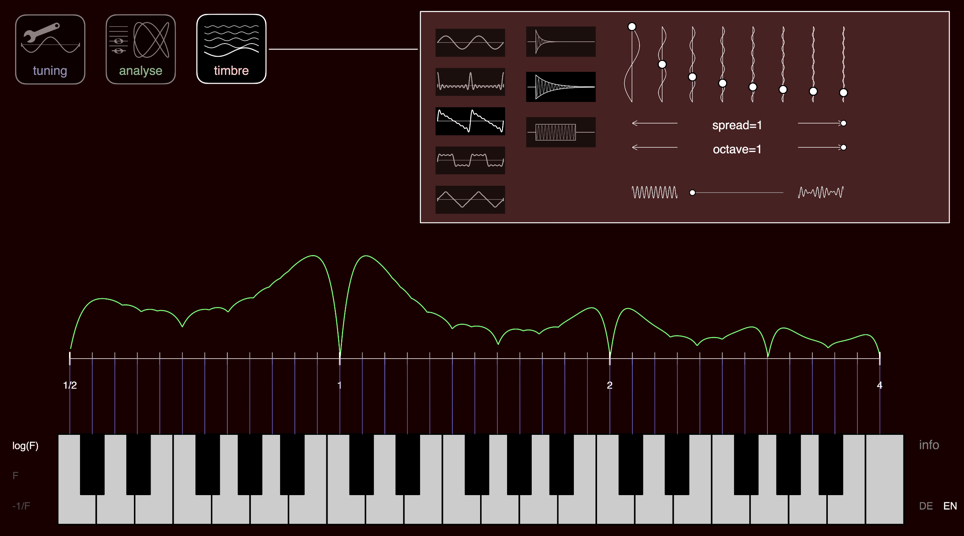
\includegraphics[width=0.9\textwidth]{ScaleLab_1}
\end{figure}

\subsection{Les eines}
Un conjunt de tres botons ens ajuden a modificar les característiques del to (timbre), a fer la selecció dels tons per l'escala (afinació) i a analitzar les propietats dels tons i les seves combinacions (anàlisis).


\subsubsection{Afinació}
Pots triar entre les escales occidentals (amb diverses afinacions), dues escales orientals (Raga, Gamelan) i disposes de dues eines més per generar escales (una amb un generador per intervals i una altra amb total llibertat).

\subsubsection{Anàlisi}
El botó d'anàlisis conté ginys que t'ajudaran a entendre l'escala o afinació que has seleccionat.

\subsubsection{Forma d'ona}
Aquest és el senyal que sents, el moviment de la membrana de l'altaveu (i dels teus timpans!) amb el temps. Tria un sinus com a timbre i prem una tecla per sentir una freqüència pura. Toca'n dos per veure la suma de les ones. Si proves diferents timbres (fets amb diverses freqüències) veuràs les diferents formes d'ona i en podràs sentir la diferència.

\subsubsection{Lissajous}
La corba de Lissajous es dibuixa amb un punt mòbil i que té una coordenada X donada per l'oscil·lació determinada per la primera tecla que prems i una coordenada Y donada per la segona. Això funciona millor amb ones sinusoidals pures com a timbre, però també crea corbes molt interessants amb timbres més complexos. Intervals més simples entre dues freqüències dibuixen figures més simples, que també són les més ``consonants''.

\subsubsection{Proporció}
Pots veure les proporcions entre les freqüències fonamentals de les notes que toques. Mira les diferents escales per veure la relació entre ràtios més simples i els intervals consonants.

\subsubsection{Corba de dissonància}
Els instruments reals no poden produir només una freqüència, sempre en fan moltes alhora (espectre). Per això la consonància o dissonància depèn de la interacció entre els grups de freqüències. Aquesta corba (basada en un concepte de Helmholtz) intenta mesurar la dissonància de cada nota respecte la nota Do central, i varia quan el timbre canvia. Veuràs que la dissonància és mínima quan hi ha un salt d'octava, de quinta o de tercera major.

\subsubsection{Timbre}
Un to produït per un instrument no sol ser una sola freqüència pura sinó una barreja de diferents freqüències amb diferents intensitats (espectre). Aquesta eina permet la selecció d'alguns espectres predefinits així com definir-ne un de propi ajustant els nivells. Totes les escales, ajusts d'afinació i anàlisis fets per altres eines es veuran influenciats pel timbre de l'instrument que decideixis tocar.

\subsection{Rerefons i Experiments}
Les següents pàgines descriuen conceptes i experiments que es poden fer utilitzant el mòdul Scale Lab.

\subsubsection{Batec}
Si dues freqüències són properes, apareix un fenomen interessant i fonamental: el volum del so sembla incrementar i disminuir periòdicament... i realment ho fa. Hi ha dues maneres d'explicar aquest efecte: assumeix que tens dues freqüències, una de 100 vibracions per segon i una altra de 101 vibracions per segon. En tot moment les dues ones se sumen. Si el pic d'una ona es troba amb la vall de l'altra una cancel·la l'efecte de l'altre. Per altra banda, si un pic coincideix amb un altre pic, la suma farà que la intensitat de la vibració total sigui el doble que la de les originals.

\begin{figure}[h]
\centering
\begin{tikzpicture}
\scriptsize
\node at (0,0) {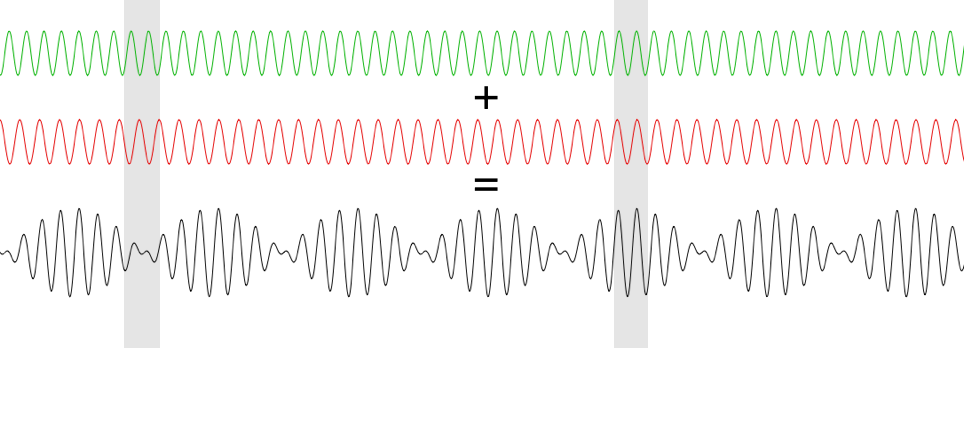
\includegraphics[width=0.9\textwidth]{ScaleLab_3_nolabels} };
\node at (-3.86,-1.6) [align=center, anchor=north]
    {Muntanya troba muntanya, \\ el senyal es fa sord.};
\node at (1.73,-1.6) [align=center, anchor=north]
    {Muntanya troba vall, \\ el senyal es fa fort.};
%\draw (-3.86,-1.6) circle [radius=0.5mm];
%\draw (1.73,-1.6) circle [radius=0.5mm];
\end{tikzpicture}
\end{figure}

La segona manera de mirar-ho és més quantitativa. Hi ha una fórmula trigonomètrica que descriu el que passa quan es sumen dues ones sinusoidals $f_1$ i $f_2$:
$$\sin(f_1 \cdot t) + \sin(f_2\cdot t) = 2 \sin\left( \frac{f_1+f_2}{2}\cdot t\right) \cdot \cos\left( \frac{f_1-f_2}{2}\cdot t\right) .$$

L'ona resultant es pot considerar com un senyal que vibra a la freqüència mitjana (la part de sinus de la dreta de l'equació) i modulada amb una baixa freqüència depenent de la diferència entre les dues freqüències originals (la part de cosinus de la dreta de l'equació). Si les freqüències són properes se sentiran canvis a freqüències baixes en la intensitat del so.

\paragraph{Experiment:} Ves a timbre i selecciona una ona sinusoidal pura. Després fes servir dos dits per generar dos tons propers. Intenta escoltar el batec. Com més properes són les freqüències més lenta serà. En canvi, si separes les freqüències, el batec es fa tan de pressa que es percep com una dissonància. Si les separes encara més acabaràs sentint dos tons diferents. Si fas servir l'eina d'ona o Lissajous podràs veure el batec representat gràficament.

\paragraph{Música:}Els batecs lents com el vibrato fan els sons més rics i una mica més orgànics. Per aquest motiu en molts instruments basen la seva generació de so en aquest fenomen. En un piano, les notes agudes solen tenir dues o tres cordes i aquestes estan lleugerament desafinades entre elles, donant lloc a un to més orgànic i ric. Un altre exemple és el mode Musette en un acordió. Aquest té dues llenguetes metàl·liques lleugerament desafinades que generen un so amb vibrato.

\subsubsection{So desde Harmònics}
Els ajusts de to del Scale Lab permeten molts més sons que les ones sinusoidals simples. Pots combinar ones sinusoidals per generar un so més complex. Els botons lliscants a la caixa de timbre et permeten afegir múltiples de la freqüència base. Si el botó lliscant de difusió està posat a 1, les freqüències utilitzades són les múltiples enteres $f$, $2f$, $3f$, $4f$, $5f$, $6f$, $7f$ i $8f$ de la freqüència base. La síntesi de Fourier implica que qualsevol senyal periòdic es pot generar per la suma ponderada d'ones sinusoidals d'aquest tipus. Per replicar perfectament un senyal et caldrien infinits sumands, però, de tota manera, les 8 freqüències que ofereix el Scale Lab ja donen un resultat prou precís.

\begin{figure}
\centering
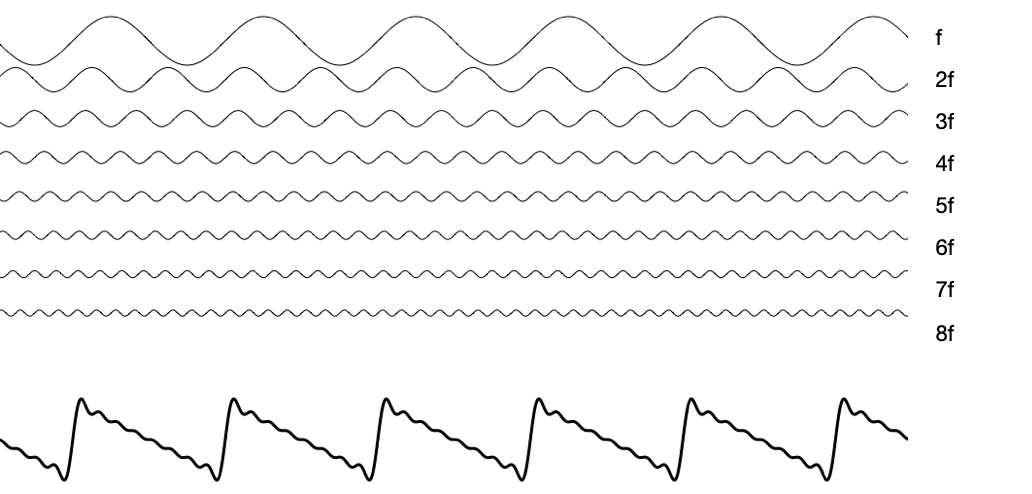
\includegraphics[width=0.9\textwidth]{ScaleLab_5}
\caption*{Aquesta imatge il·lustra com la suma d'harmònics amb intensitats 1, 1/2, 1/3, 1/4, ... resulta en una funció periòdica amb forma de dents de serra.}
\end{figure}

\paragraph{Experiment:}
Ves a timbre i experimenta amb les diferents models predefinits de forma d'ona (els botons de l'esquerra). Mou els botons lliscants per cada harmònic per veure com canvia el so. Pots fer servir l'eina d'anàlisis per veure les formes d'ona que has generat.

\paragraph{Music:}
És un fet que el so de molts instruments (particularment els de corda, vent-metall o vent-fusta) s'aproximen fàcilment amb la descomposició del seu so en harmònics. Això té relació amb les físiques específiques dels instruments.

\begin{figure}
\centering
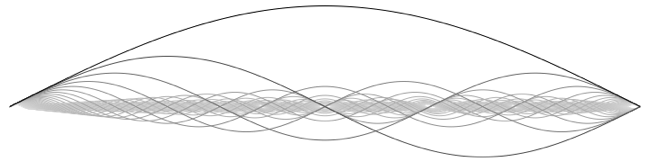
\includegraphics[width=0.9\textwidth]{ScaleLab_6}
\caption*{La imatge mostra les ones parcials d'una corda ideal vibrant. Corresponen exactament als harmònics, resultant en un so que pot modelar-se molt bé amb aquesta aproximació.}
\end{figure}


\subsubsection{Parcials dispersos}
El món no és un laboratori ideal. Les físiques són complexes i els sons no són sumatoris perfectes d'harmònics. De fet, molts instruments creen sons on les freqüències més altes no encaixen amb els harmònics. Per exemple, el fet que una corda no sigui infinitament prima resulta en una certa desviació de la sèrie ideal d'harmònics. Com més gruixut és el material que vibra més extrema es torna la desviació respecte a la sèrie d'harmònics ideals. L'espectre d'una campana d'església és substancialment diferent  d'una sèrie d'harmònics. Això no és dolent. Fa els sons més rics, més únics o més característics. A continuació pots veure el que passa si se substitueix un espectre d'harmònics per un de dispersió on les freqüències segueixen la norma
$$1^af, 2^af, 3^af, 4^af, 5^af, 6^af, 7^af, 8^af$$
Per un exponent $a$ petit. Fixa't que la suma resultant dels parcials (que és el nom adient en aquest cas) mostra un comportament constantment variant a la corba sonora resultant i ja no és periòdica. Aquest so resultant és més ric i orgànic.

\paragraph{Experiment:}
A la caixa de timbre del Scale Lab hi ha un botó lliscant anomenat dispersió just a sota dels botons lliscants dels harmònics. Juga amb aquest botó lliscant per experimentar amb espectres dispersos o comprimits. Escolta com canvia el so amb petites dispersions. Analitza el so resultant amb l'eina ona per veure com en canvia la forma. Com sonen els intervals ara? Quines són les diferències entre baixa i alta dispersió? I entre dispersió i compressió de l'espectre? Hi ha un món de possibilitats per descobrir.

\subsubsection{Corbes de Dissonància}
Tan bon punt dos tons (amb un cert espectre de parcials) es reprodueixen alhora els nostres cervells comencen a categoritzar els intervals en un cert rang entre sons agradables (consonants) i no tan agradables (dissonants). Podríem pensar que l'art de la música és l'art de crear la tensió adequada entre consonància (per agradar a la gent) i dissonància (per fer-ho més interessant). De fet, diferents èpoques i cultures tenen opinions molt diverses sobre el que es considera bon gust, però el concepte global preval.

\begin{figure}[h]
\centering
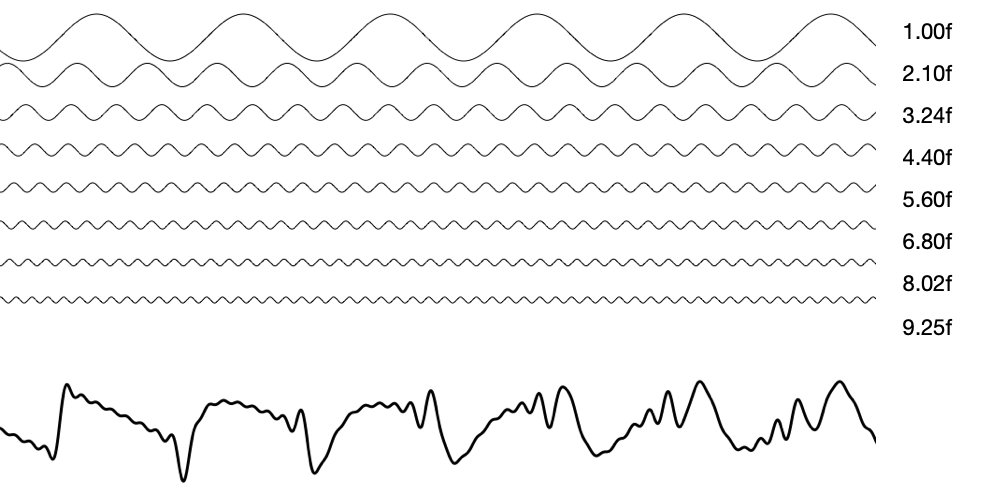
\includegraphics[width=0.9\textwidth]{ScaleLab_7}
\caption*{Hi ha una altra interpretació de la riquesa del so que està guanyant popularitat. Com que els parcials no es corresponen perfectament amb els harmònics, quan es toquen intervals, hi ha un batec irregular i substancial a les freqüències altes.}
\end{figure}

Ja al voltant de l'any 1870, Hermann von Helmholtz va desenvolupar la teoria matemàtica de la consonància i dissonància. La idea al darrere és tan simple com brillant. Com que sempre que es toquen dos tons alhora molts parcials sonen en el mateix moment, el que cal fer és sumar les dissonàncies entre els parells involucrats d'ones sinusoidals per obtenir la dissonància del so total. D'aquesta manera, ell va reduir la pregunta sobre dissonància de sons complexos a dissonància entre ones sinusoidals. (Ens podem preguntar si és una assumpció raonable, però almenys és un bon punt de partida). De tota manera, què és la dissonància entre dues ones sinusoidals? Aquí calen dades empíriques. Resulta que si les ones són més o menys de freqüència idèntica els batecs no es perceben com si fossin dissonants. Un batec petit, de baixa freqüència, fins i tot és agradable. Per altra banda, tan bon punt el batec es torna massa ràpid es percep com a aspre i dissonant. Aquest efecte és particularment fort amb batecs d'entre 10 i 25 cops per segon, després l'efecte disminueix una altra vegada. Si els tons estan massa separats es senten com a dues ones sinusoidals independents. A continuació podeu veure la corba de dissonància d'una ona sinusoidal afinada en un Do central.

\begin{figure}[h]
\centering
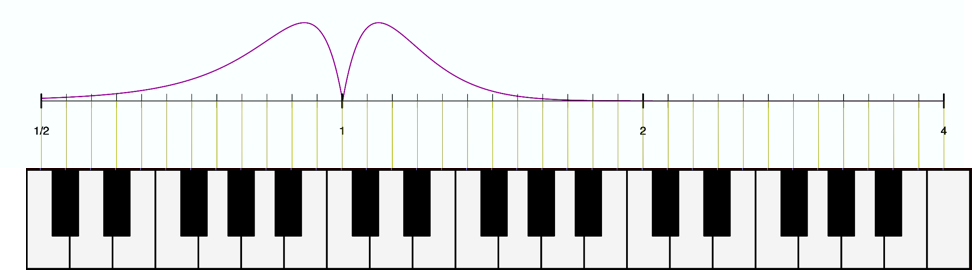
\includegraphics[width=0.9\textwidth]{ScaleLab_9}
\end{figure}

Les coses es posen interessants tan bon punt l'espectre es torna complicat. La següent imatge mostra corba de dissonància resultant d'un ric espectre harmònic. Les dissonàncies entre harmònics dels dos tons generats generen els màxims i mínims característics d'aquestes corbes. Fixa't que la dissonància és mínima als harmònics que componen l'octava, la quinta, la quarta i la tercera.

\begin{figure}[h]
\centering
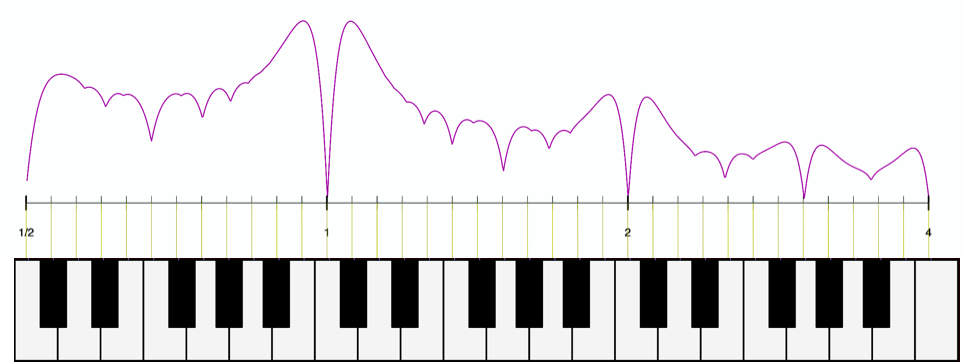
\includegraphics[width=0.9\textwidth]{ScaleLab_10}
\end{figure}

\paragraph{Experiment:}
Comença l'analitzador de corbes dissonants i toca intervals amb el Do central. Juga amb diferents timbres i experimenta amb diferents intervals. La teva percepció coincideix amb la predicció?

\subsubsection{Dissonància i Parcials Dispersos}
Què passa si estudiem el comportament dissonant d'un espectre de parcials dispersos? El comportament de la dissonància ve fortament determinat per la dissonància entre harmònics o parcials. En conseqüència, en el moment que els parcials estiguin ``fora de lloc'' aconseguim un nou comportament dissonant.
La següent imatge mostra el que passa amb un espectre de parcials lleugerament dispersos.($a=1.08$):

\begin{figure}[h]
\centering
\begin{tikzpicture}
\scriptsize
\node at (0,0) {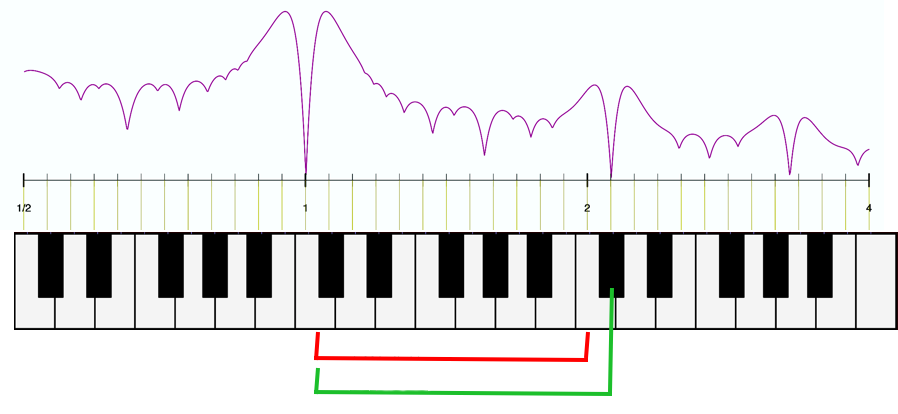
\includegraphics[width=0.9\textwidth]{ScaleLab_11_nolabels} };
\node at (-1,-1.65) [align=left, anchor=west]
    {dissonància};
\node at (-1,-2.08) [align=left, anchor=west]
    {consonància};
%\draw (-1,-2.05) circle [radius=0.5mm];
\end{tikzpicture}
\end{figure}

Per un músic acostumat al nostre clàssic sistema de tons el resultat pot ser impactant. De cop i volta els intervals que solen sonar consonants (com l'octava) sonen marcadament dissonants. Per altra banda, altres que solien sonar molt dissonants (com la petita novena entre el do i el do sostingut) sonen preciosos.

Per tant, els instruments que generen un espectre dispers o comprimit requereixen un tipus diferent d'escales. O, dit d'altra manera, el nostre sistema tonal occidental està fortament influenciat pel fet que els instruments més habituals són de cordes, vent-metall o vent-fusta.

Hi ha una cura molt senzilla per arreglar les octaves dissonants: separar les freqüències de l'escala igualment! Després de fer-ho l'octava ja no serà una octava, però sonarà com si en fos una.

\begin{figure}[h]
\centering
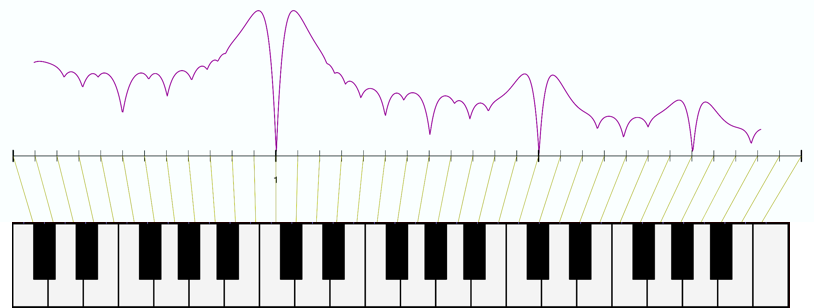
\includegraphics[width=0.9\textwidth]{ScaleLab_12}
\end{figure}

\paragraph{Experiment:}
Els següents experiments poden ser sorprenents. Encén l'analitzador de corbes de dissonància i toca intervals amb el Do central. Experimenta amb la dispersió de l'espectre i amb la dispersió de l'octava. Si disperses els dos elements en la mateixa mesura tindràs una experiència tonal molt similar a l'habitual.

\paragraph{Music:}
En alguns casos, pot ser una bona pràctica dispersar les escales. Si dissenyes les campanes d'un campanar d'església adaptant l'escala a un espectre, és una bona idea. Fins i tot un piano normal sona més brillant si les octaves estan lleugerament dispersades. De tota manera, per aquest piano amb escales dispersades serà complicat tocar amb altres instruments. La música està plena de compromisos.

\subsubsection{Sistemes d'Afinació Occidentals}
Hem vist que el timbre i les freqüències dels parcials influeixen al comportament dissonant dels intervals. En conseqüència, la selecció de tons (l'escala) utilitzada en un instrument ha de dependre de les característiques sonores d'aquest. Els instruments de la cultura occidental (arpes, pianos, flautes, trompetes...) tenen un espectre gairebé perfecte en el sentit que els parcials són molt propers als harmònics teòrics. Per això, les ràtios de freqüència de $2 : 1$ (octava), $3 : 2$ (quinta), $4 : 3$ (quarta), $4 : 5$ (tercera major) i $6 : 5$ (tercera menor) donen lloc a intervals relativament consonants (escrits en ordre decreixent).

Resulta que les quintes, quartes (música Gregoriana), i les terceres modernes (barroques) i altres intervals dissonants encara més moderns (impressionistes, expressionistes) van entrar al llenguatge musical de la cultura occidental.

Quina és una bona selecció de tons per aquesta música? Quines són bones escales? Respondre aquestes preguntes en profunditat podria donar lloc a una assignatura universitària d'un any sencer. Nosaltres només  en veurem una introducció.

Sistema de 12 tons: els sistemes occidentals actuals amb 12 tons per octava són els més habituals. La raó d'això és matemàtica. Agrupar 12 quintes perfectes ens porta a gairebé crear 7 octaves. Vist en una fórmula:
$$\left( \frac{3}{2}\right)^{12} = 129.7463 \ldots \approx 2^7 = 128 .$$

Els 12 intervals són el primer sistema en què els conjunts s'apropen a una relació d'octava. Si algú volgués un sistema tonal centrat en octaves i quintes, el sistema de 12 tons és un bon punt de partida.

Per desgràcia, aquesta relació no és perfecta i aquí és on tota la història dels sistemes d'afinació comença: s'han de fer compromisos i les diferents èpoques han resolt aquesta tensió de maneres diferents.

\begin{figure}[h]
\centering
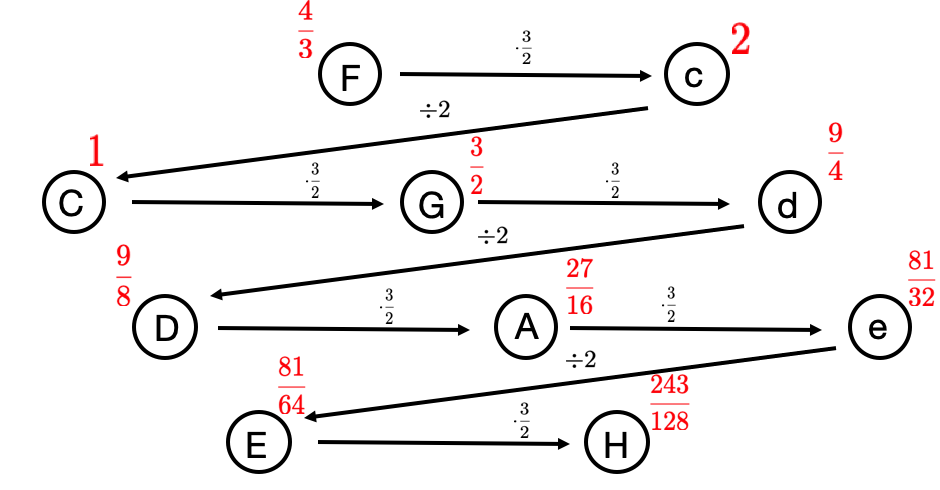
\includegraphics[width=0.7\textwidth]{ScaleLab_14}
\caption*{Afinació Pitagòrica}
\end{figure}

Afinació Pitagòrica: comencem amb l'afinació Pitagòrica, que se centra al voltant de la idea de tenir tantes quintes perfectes com sigui possible. Fixa't en els set tons de l'escala de Do major i mira el que passa. Etiquetem els tons per ràtio de freqüència amb relació al Do i dividim per 2 (baixem una octava) cada vegada que aquesta relació esdevé major que 2. Els següents diagrames mostren les ràtios de les notes a l'escala pitagòrica i com es deriven.

Totes les quines i octaves en aquest sistema són perfectes. Tot i això, fixa't que al Mi se li assigna una freqüència de 81/64. Això no és una tercera major perfectament afinada, la tercera perfecta seria $5/4=80/64$.

Per això la tercera pitagòrica està desafinada per un factor de 81/80 respecte de la tercera perfecta. El més probable és que Pitàgores no li donés gaire importància a les terceres, ja que van començar a ser rellevants cap a 1500 anys després. Com s'ha comentat abans, no totes les quintes poden ser perfectes. Si tinguéssim 11 quintes perfectament afinades, l'última sonaria realment malament.

Afinació justa: considerem ara una afinació que es centra en quintes i terceres. Aquesta s'anomena afinació justa. Per les 7 notes de l'escala de Do major utilitza el següent esquema d'afinació:

\begin{figure}[h]
\centering
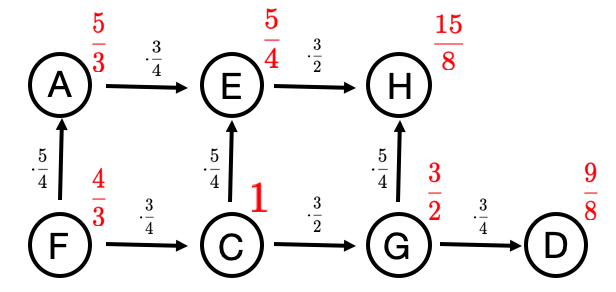
\includegraphics[width=0.7\textwidth]{ScaleLab_15}
\caption*{Afinació justa}
\end{figure}

Pots tocar un munt de terceres i quintes perfectes amb aquesta afinació, però en perds d'altres. Aquesta petita quadrícula que acabes de veure és una petita porció del Tonnetz.


Afinació de temperament igual: si extens tant l'afinació pitagòrica com l'afinació justa als 12 semitons, alguns intervals seran perfectes, però d'altres no sonaran tan bé. L'aproximació moderna a l'afinació consisteix q evitar això mitjançant la dispersió igualitària de l'error sobre tots els intervals. (Això es pot considerar com una mena d'aproximació democràtica a l'afinació). En l'afinació de temperament igual una octava es divideix en 12 semitons idèntics. Cada semitò multiplica la seva freqüència per un factor de $\sqrt[12]{2}$ i això permet arribar a una octava perfecta precisament cada 12 esglaons. Amb aquest mètode, totes les quintes arrosseguen el mateix error i el mateix passa a la resta d'acords i intervals. A continuació es comparen els valors de l'afinació de temperament igual amb els de l'afinació perfecta:
$$\textrm{for fifth: } (\sqrt[12]{2})^7 = 1.498\ldots \approx 1.5 = \frac{3}{2} ,$$
$$\textrm{for thirds: } (\sqrt[12]{2})^4 = 1.26\ldots \approx 1.25 = \frac{5}{4} .$$
S'observa que aquestes aproximacions són molt bones.

\paragraph{Experiment:}
Obre la caixa d'afinacions i experimenta amb diferents afinacions occidentals. Els colors que mostra el Tonnetz indiquen com són de propers els intervals de l'escala seleccionada als perfectes. És molt instructiu analitzar les diferents afinacions amb l'eina ràtio. Aquesta mostra les ràtios dels intervals si aquests es toquessin al teclat. La fotografia següent mostra les ràtios de freqüència per un acord de Do major.

\begin{figure}[h]
\centering
\begin{tikzpicture}
\scriptsize
\node at (0,0) { 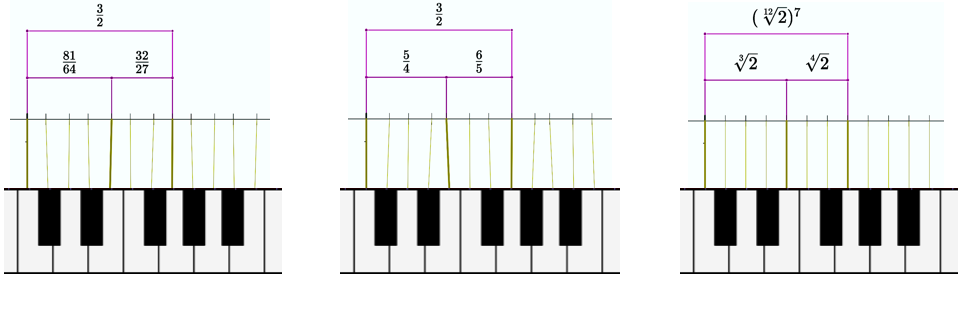
\includegraphics[width=0.95\textwidth]{ScaleLab_18_nolabels} };
\node at (-5.75,-1.65) [align=left, anchor=west]
    {Afinació pitagòrica};
\node at (-1.65,-1.65) [align=left, anchor=west]
    {Afinació justa};
\node at (2.5,-1.65) [align=left, anchor=west]
    {Afinació de temperament igual};
\end{tikzpicture}
\end{figure}

\subsubsection{Escales Raga Índies}
Hi ha una altra manera de tocar terceres i quintes perfectes: afegir més tons a l'escala! Els sistemes d'afinació per la Música Raga Índia utilitzen aquest mètode. A grans trets, aquests sistemes d'afinació es poden caracteritzar amb el següent esquema:

\begin{figure}[h]
\centering
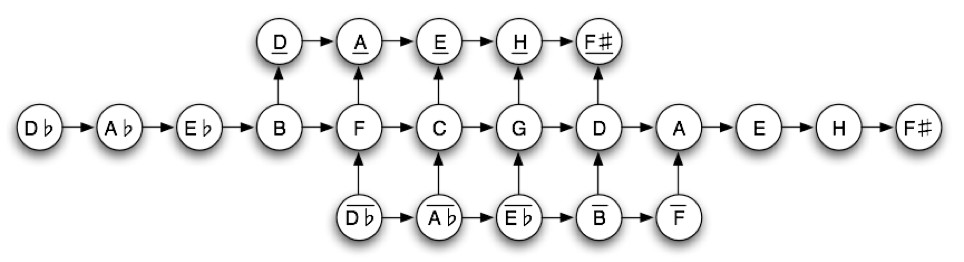
\includegraphics[width=0.9\textwidth]{ScaleLab_19}
\end{figure}

Cada fletxa horitzontal indica (fins al salt d'octava) una octava perfecta i cada fletxa vertical una tercera perfecta. A diferència de la música occidental, la música Raga té una tradició més oral que escrita. Per aquest motiu, és força difícil d'aconseguir un sistema concret d'afinació, però el sistema que es descriurà que consisteix en 22 tons s'accepta per la majoria de persones que han analitzat la música índia. Llavors, què és tan especial i interessant sobre aquest sistema d'afinació i per quin motiu hi ha exactament 22 tons?

Per començar, cal adonar-se que les Ragues índies sempre es refereixen a un to base. Normalment un interval es toca constantment de fons, com un brunzit. El més habitual és el Do-Sol. Fixa't com aquest interval és el centre de simetria del diagrama anterior.

La fila central del diagrama és l'escala pitagòrica amb 11 quintes perfectes. Ara es saturen amb l'addició de les terceres perfectes, cosa que es fa molt enginyosament. Per veure-ho reordenem les notes de l'escala pitagòrica per formar una cadena de semitons. Obtenim:

\begin{figure}[h]
\centering
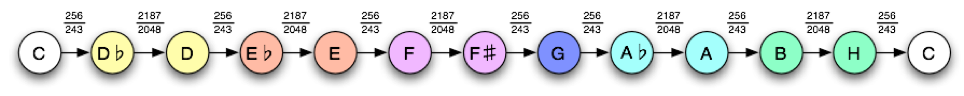
\includegraphics[width=0.95\textwidth]{ScaleLab_21}
\end{figure}

Les ràtios entre els tons representen les ràtios de freqüències que vénen de l'afinació pitagòrica.

Pots observar com, gairebé de forma màgica, només apareixen dos tipus de fraccions. Els colors al diagrama marquen la més gran de les fraccions, per tant tenim salts grans i petits de semitons. Dos tons relacionats per un salt gran tenen el mateix color. Ara es pot dividir l'interval de 2187/2048 restant de forma elegant afegint dues noves notes.

\begin{figure}[h]
\centering
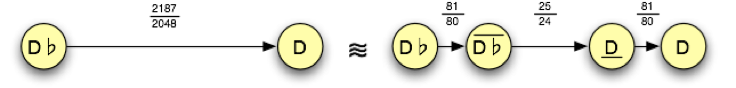
\includegraphics[width=0.95\textwidth]{ScaleLab_22}
\end{figure}

A l'exemple anterior s'observa que s'obté una versió més aguda del Re bemoll i una versió més greu del Re. Aquestes són exactament les dues noves notes afegides amb el sistema mencionat. Ara podem fer una divisió similar per tota la resta de salts grans de semitò. Això resulta en un sistema amb 22 tons, mostrats amb colors al següent esquema del sistema tonal:

\begin{figure}[h]
\centering
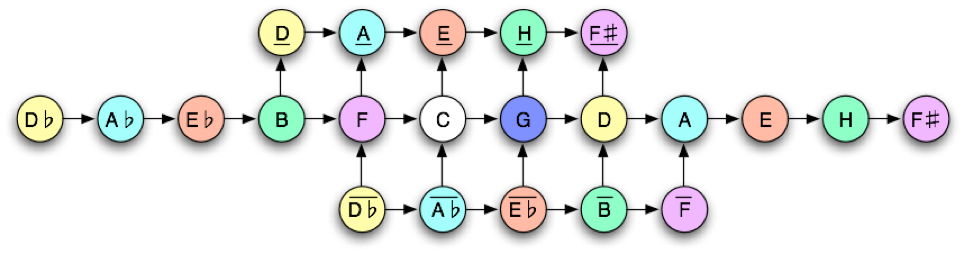
\includegraphics[width=0.95\textwidth]{ScaleLab_20}
\end{figure}


Fixa't que el Do i el Sol juguen un paper especial en aquest sistema, ja que són les úniques notes que no es veuen involucrades en aquesta divisió dels intervals.

Els tons del sistema d'afinació Raga es diuen Shrutis. Tal com es fa amb les afinacions occidentals, sovint les melodies no utilitzen tots els tons alhora. En comptes d'això se seleccionen algunes notes per formar escales més petites basades en aquest sistema més gran. La selecció d'aquestes subescales (normalment d'entre 4 i 7 tons) també segueixen certes normes, però no s'entrarà en tant detall aquí.

\paragraph{Experiment:}
Obre la caixa d'afinació i experimenta amb els sons de les afinacions Raga. Pots seleccionar un munt de subescales usualment utilitzades amb el sistema de 22 tons. També pot ser interessant mesurar les ràtios de freqüència entre els tons.

\begin{sectcredits}
\item[Autor del mòdul:] Jürgen Richter-Gebert (Technical University of Munich).

\item[Agraïments:] Patrick Wilson i Aaron Montag (sistema de so). Basat en CindyJS.org

\item[Text:] Jürgen Richter-Gebert (TU Munich).
\end{sectcredits}
